\newcommand{\plB}{\plfoo{B}}
\newcommand{\plE}{\plfoo{E}}

\thasse{
	\begin{frame}{}
		\begin{block} {Aussagenlogik}
			\begin{itemize}
				\item \enquote{Es regnet und alle Vögel sind grau.}
				\item atomar: \enquote{Es regnet.}, \enquote{ Alle Vögel sind grau.}
				\item Diese beiden Aussagen lassen sich ihrerseits nicht in weitere Teilaussagen zerlegen!
			\end{itemize}
		\end{block}
		
		\pause
		\begin{block} {Prädikatenlogik}	
			\begin{itemize}
				\item In der Prädikatenlogik werden atomare Aussagen hinsichtlich ihrer inneren Struktur untersucht.
				\item \enquote{Alle Vögel sind grau}
				\item lässt sich in : \enquote{Alle Vögel}, \enquote{sind grau} zerlegen.
			\end{itemize}
			
		\end{block}
	\end{frame}
}

\section{Prädikatenlogik: Syntax}



\begin{frame}{Syntax}
	\begin{block}{Aufbau von prädikatenlogischen Formeln}
	\begin{itemize}[<+->]
		\item \textbf{Terme}: Liefern \enquote{Werte} (Zahlen, Wörter, whatever...); \\ 
		Aus Konstanten, Variablen und Funktionssymbolen zusammengesetzt.
		\item \textbf{Atomare Formeln}: Liefern Wahrheitswerte $\in \BB$; \\
		 Aus Termen und Relationssymbolen zusammengesetzt.
		\item \textbf{Prädikatenlogische Formeln}: aus atomaren Formeln und AL-Konnektiven sowie Quantoren ($\forall, \exists$) zusammengesetzt. 
	\end{itemize}
	\end{block}
\end{frame}

\begin{frame}{Terme}
	Bestehen aus... \\
	\medskip
	
	\textbf{Variablen} \, (endlich viele) \quad Alphabet $\VPL$ \\
	$\word{x}_i$ \quad $\word x, \word y, \word z$ \\
	Können in einer Formel beliebig verschiedene Werte annehmen \\
	\medskip \pause
	
	\textbf{Konstanten} \, (endlich viele) \quad Alphabet $\CPL$ \\
	$\word{c}_i$ \quad $\word c, \word d$ \\
	Konstanter Wert in der gesamten Formel \\
	\medskip \pause
	
	\textbf{Funktionen} \, (endlich viele) \quad Alphabet $\FPL$ \\
	$\word{f}_i$ \quad $\word f, \word g, \word h$ \\
	Liefern Werte für irgendwelche Eingaben (wie gewohnt) \\
	Jedes $\word{f}_i$ hat Stelligkeit $\ar(\word{f}_i) \in \N_+$ \quad „Wieviel Argumente $\word{f}_i$ nimmt“ {\small (Arität)} \\
	\smallskip \pause
	
	Beispiel: 
	\quad Funktionen $\word f$ mit $\ar(\word f) = 2$, \quad $\word g$ mit $\ar(\word g) = 1$. \\ \pause
	\quad OK: \qquad \word{f(x,y)} \qquad \word{g(c)} \qquad \word{g(f(x,c))} \\
	\quad Kaputt: \qquad \word{f(c)} \qquad \word{g(x,y,z)} \qquad \word{f(x,y} \qquad \word{f(x,,}
\end{frame}

\begin{frame}{Atomare Formeln}
	Bestehen aus... \\
	\medskip
	
	\textbf{Termen} (von eben) \\
	\medskip
	
	\textbf{Relationen} \, (endlich viele) \quad Alphabet $\RPL$  \\
	$\pleq$ und beliebige $\word R_i$ \quad $\word R, \word S$ \\
	Liefern Wahrheitswerte in $\BB = \set{\W, \F}$ \\
	Haben auch Stelligkeit $\ar(\word R_i) \in \N_+$ \\
	\medskip \pause
	
	Beispiele: \quad Relationen \word R mit $\ar(\word R) = 1$, \quad \word S mit $\ar(\word S) = 2$ \\
	\quad $\word x \pleq \word c$ \qquad $\word{g(x)} \pleq \word{g(y)}$ \qquad $\word{R(g(c))}$ \qquad $\word{S(x,f(x,y))}$
	\medskip \pause
	
	Relationen und Funktionen können \textbf{nur mit Termen} aufgerufen werden! \\
	\impl \quad $\word x \pleq \word{(}\word y \pleq \word z\word{)}$ \qquad \word{g(S(x))} \qquad \word{R(S(x,y))} \qquad $\word{R(x)} \pleq \word{S(x,y)}$ \\
	Alles \textbf{falsch}!
\end{frame}

\begin{frame}{Prädikatenlogische Formeln}
	Bestehen aus... \\
	\medskip
	
	\textbf{Atomaren Formeln} (von eben) \\
	\medskip
	
	\textbf{AL-Konnektiven} \\
	$\alnot, \aland, \alor, \alimpl$ und Klammern {\small (einsparbar)} \\
	Verknüpfen PL-Formeln \\
	\medskip \pause
	
	\textbf{Quantoren} \\
	$\plall$ All-Quantor \quad $\plexist$ Existenz-Quantor \\
	Verwendung: $\bleftBr\plall \word x_i \text{...Formel...}\brightBr$ \quad $\bleftBr\plexist \word x_i \text{...Formel...}\brightBr$ \\
	\impl NUR \textbf{Variablen} können quantifiziert werden! \\
	\medskip 
	
	Klammerregeln: Wie bei AL-Formeln; Quantoren binden stärker als alles andere.
	\bigskip \pause
	
	\textbf{Falsch}: \\
	$\bleftBr\plexist \word c \text{...Formel...}\brightBr$ mit $\word c \in \CPL$ \quad \word c keine Variable! \\
	$\bleftBr\plall \word x \word{:} \text{...Formel...}\brightBr$ \quad KEINE Doppelpunkte! \\
\end{frame}

\begin{frame}{Aufgabe 1 (WS 15/16, Blatt 7)}
	Es seien $\CPL = \{ \}$, $\VPL = \{ \plx, \ply, \plz \}$, $\FPL = \{ \}$ und $\RPL = \{ \plE, \pleq \}$ mit $\ar(\plE) = 2$, und es sei $F$ die prädikatenlogische Formel
	\begin{equation*}
	\alnot \plexist \plx
	{\plka
		\plE{\plka \plx \plcomma \ply \plkz}
		\alor
		\alnot \plall \plz \plall \plx \plall \ply
		{\plka
			\plE{\plka \plx \plcomma \plz \plkz} \aland \plE{\plka \ply \plcomma \plz \plkz} \alimpl \plx \pleq \ply
			\plkz}
		\plkz}
	\end{equation*}
	
	\begin{block}{Aufgabe 1}
		Ist diese prädikatenlogische Formel syntaktisch korrekt?\\ \pause
		Ja
	\end{block}
\end{frame}

\mycomment{ % LEGACY. Kann wohl weg.
	\begin{frame}{Terme - Alphabet}
	\begin{figure}
		\centering
		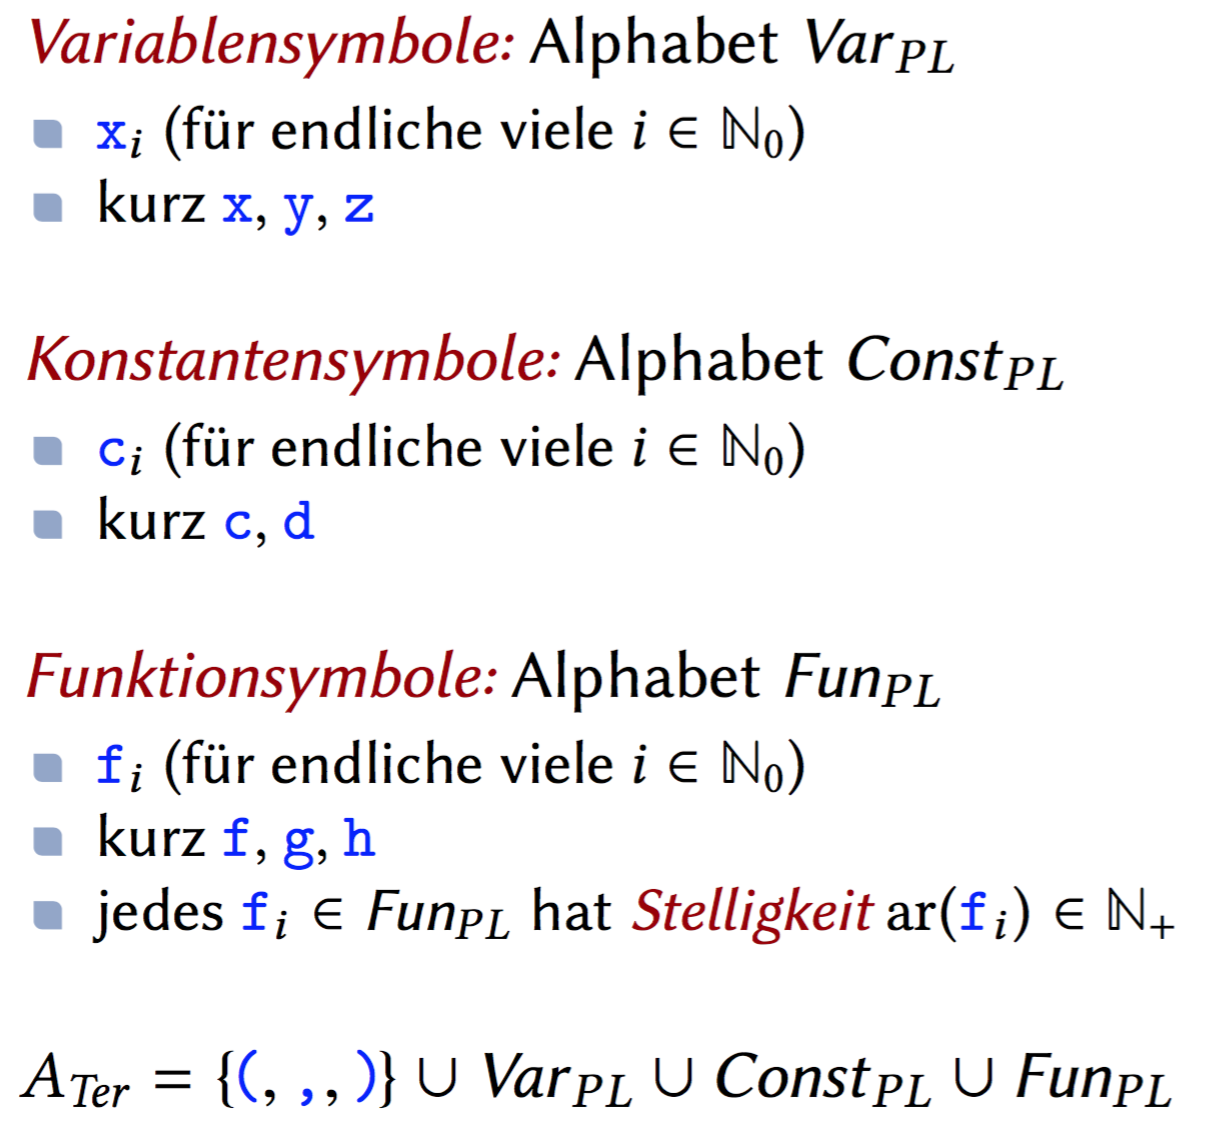
\includegraphics[scale=0.2]{pl/TermeAlphabet.png} \hspace{2em} 
	\end{figure} 
	\end{frame}
	
	\begin{frame}{Terme - Grammatik}
	\begin{figure}[h!]
		\centering
		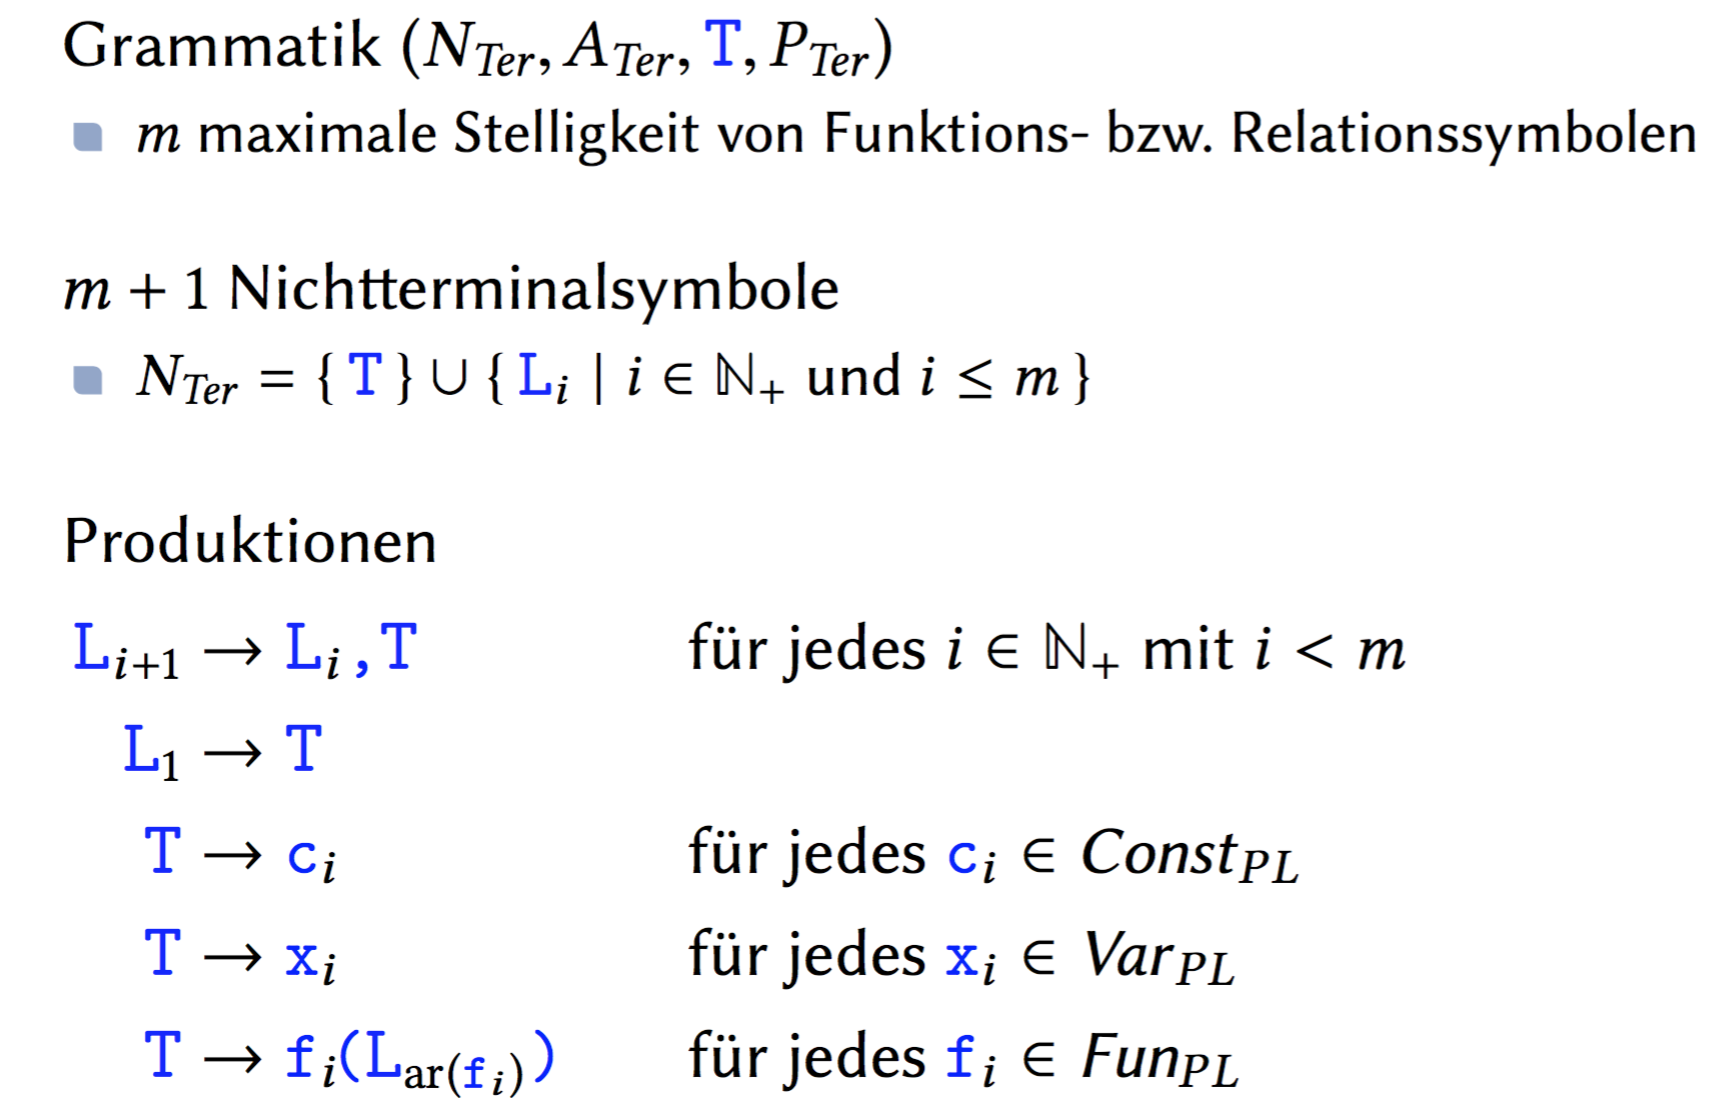
\includegraphics[scale=0.2]{pl/TermeGrammatik.png} \hspace{2em} 
	\end{figure} 
	\end{frame}
	
	\begin{frame}{Atomare Formeln}
	\begin{figure}[h!]
		\centering
		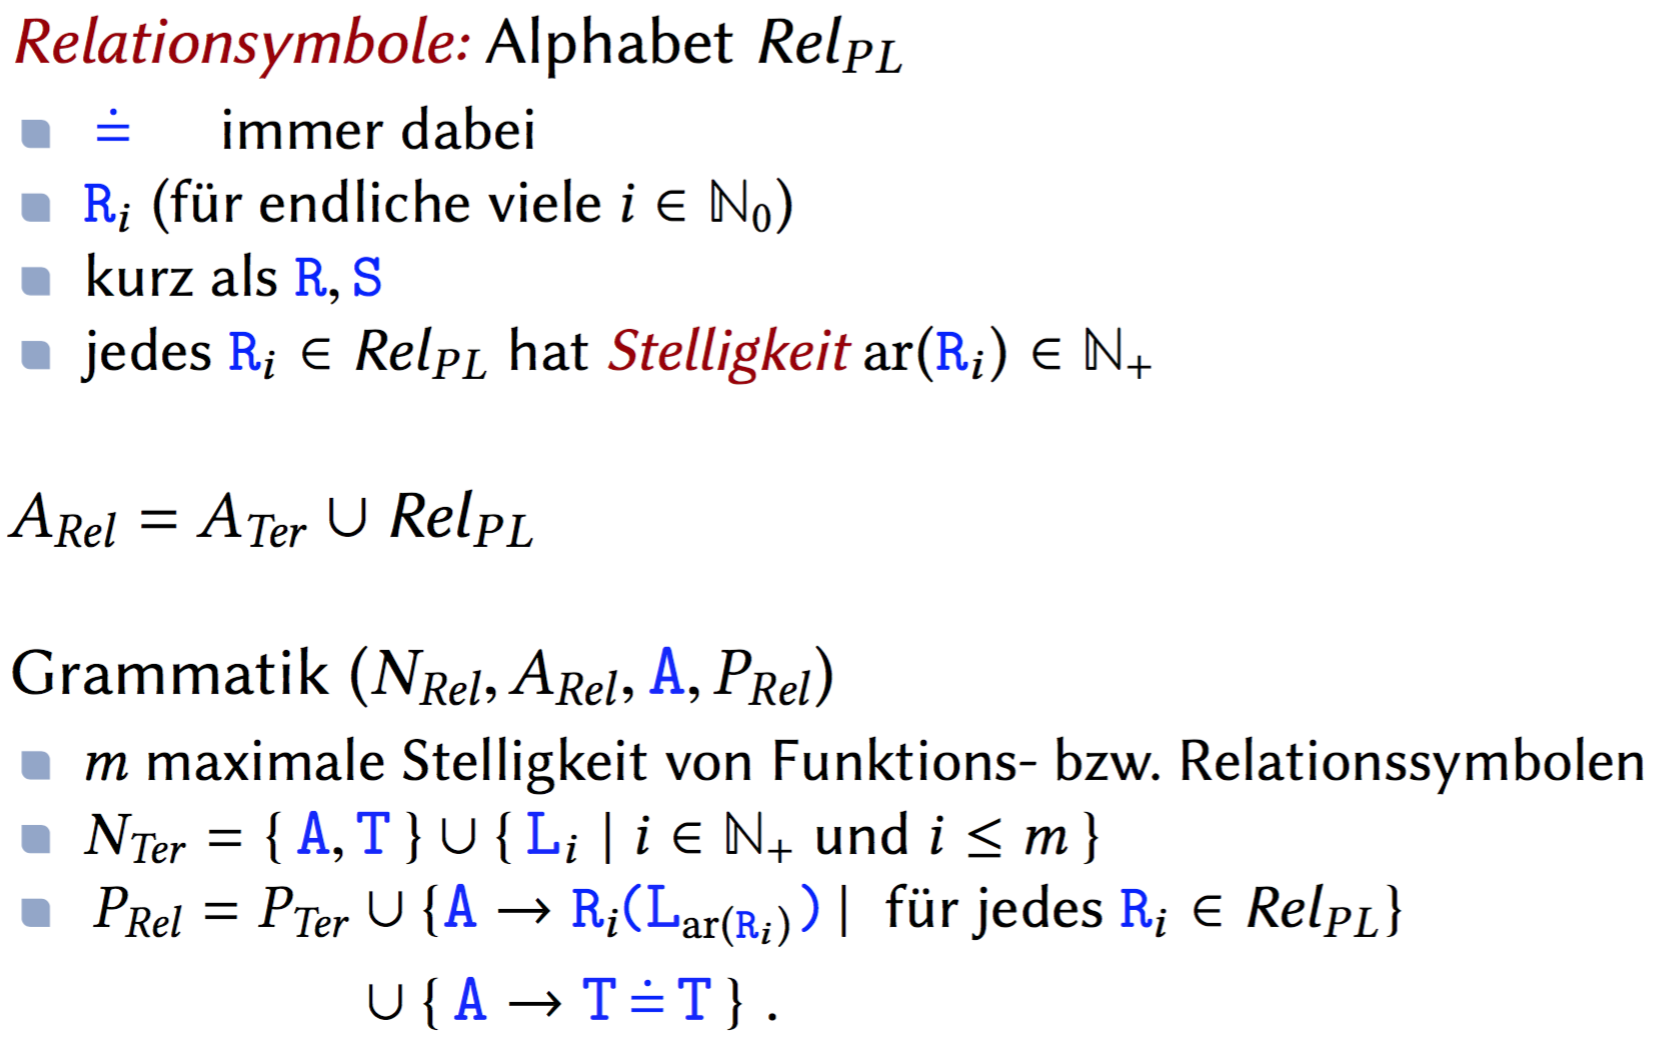
\includegraphics[scale=0.2]{pl/AFormeln.png} \hspace{2em} 
	\end{figure} 
	\end{frame}
	
	\begin{frame}{Atomare Formeln - Beispiel}
	\begin{figure}[h!]
		\centering
		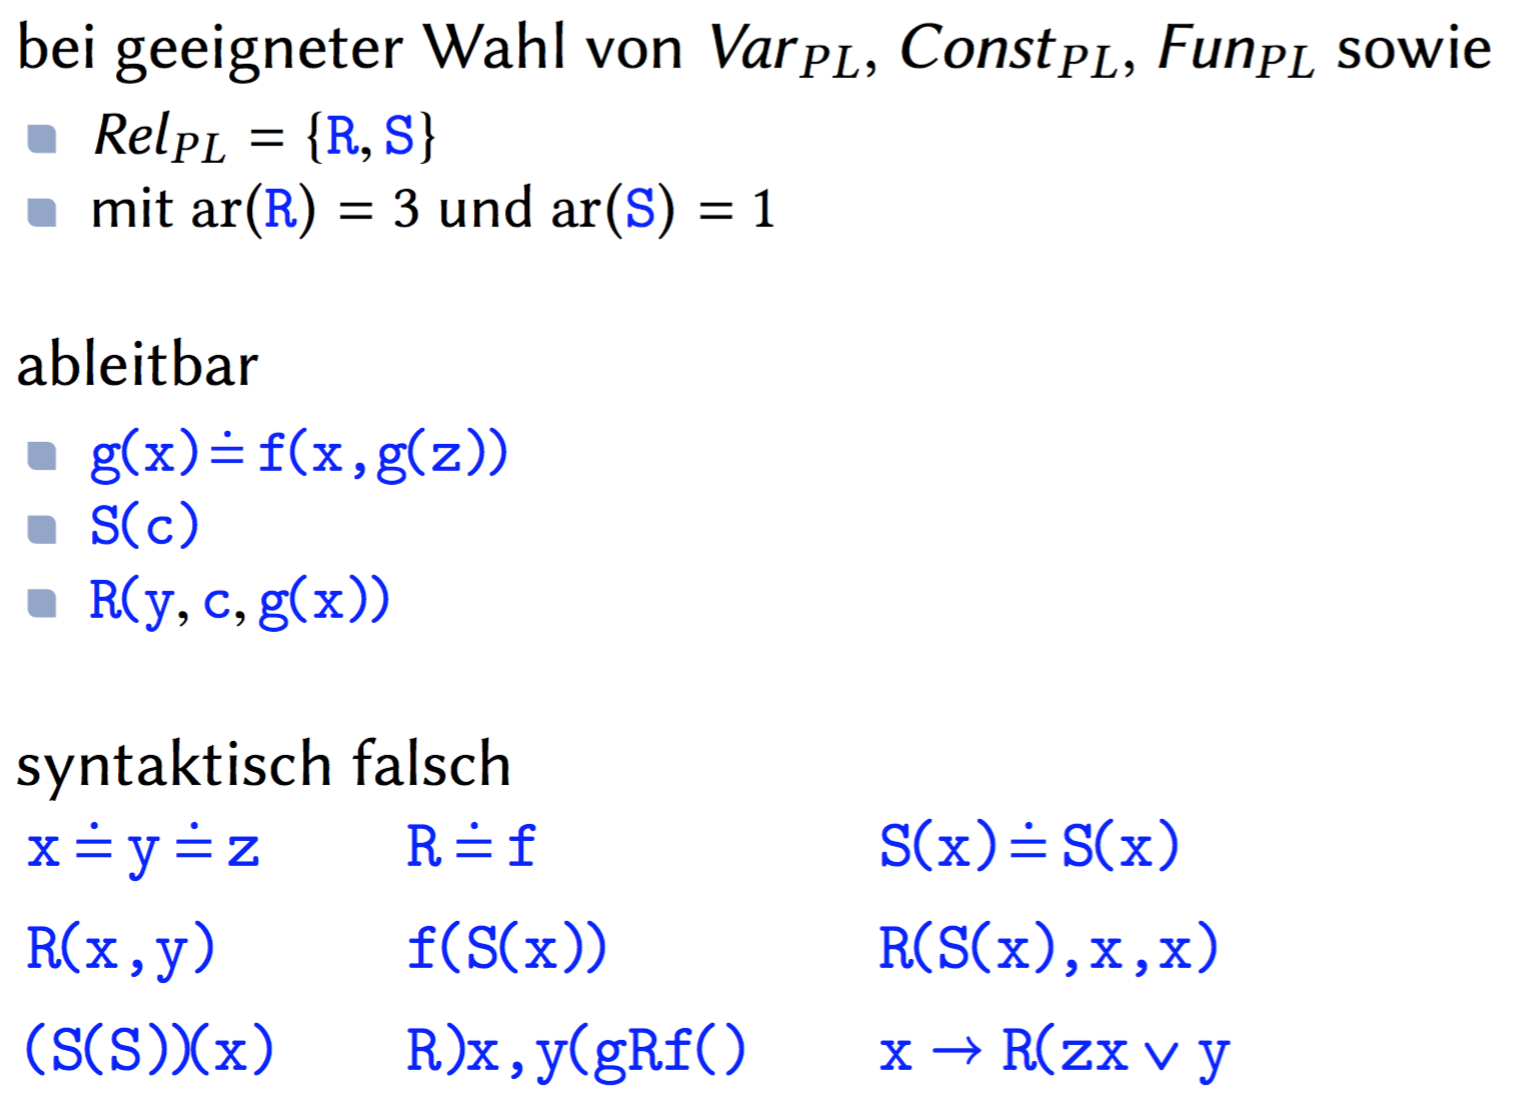
\includegraphics[scale=0.2]{pl/AFormelnBsp.png} \hspace{2em} 
	\end{figure} 
	\end{frame}
	
	\begin{frame}{Prädikatenlogische Formeln}
	\begin{figure}[h!]
		\centering
		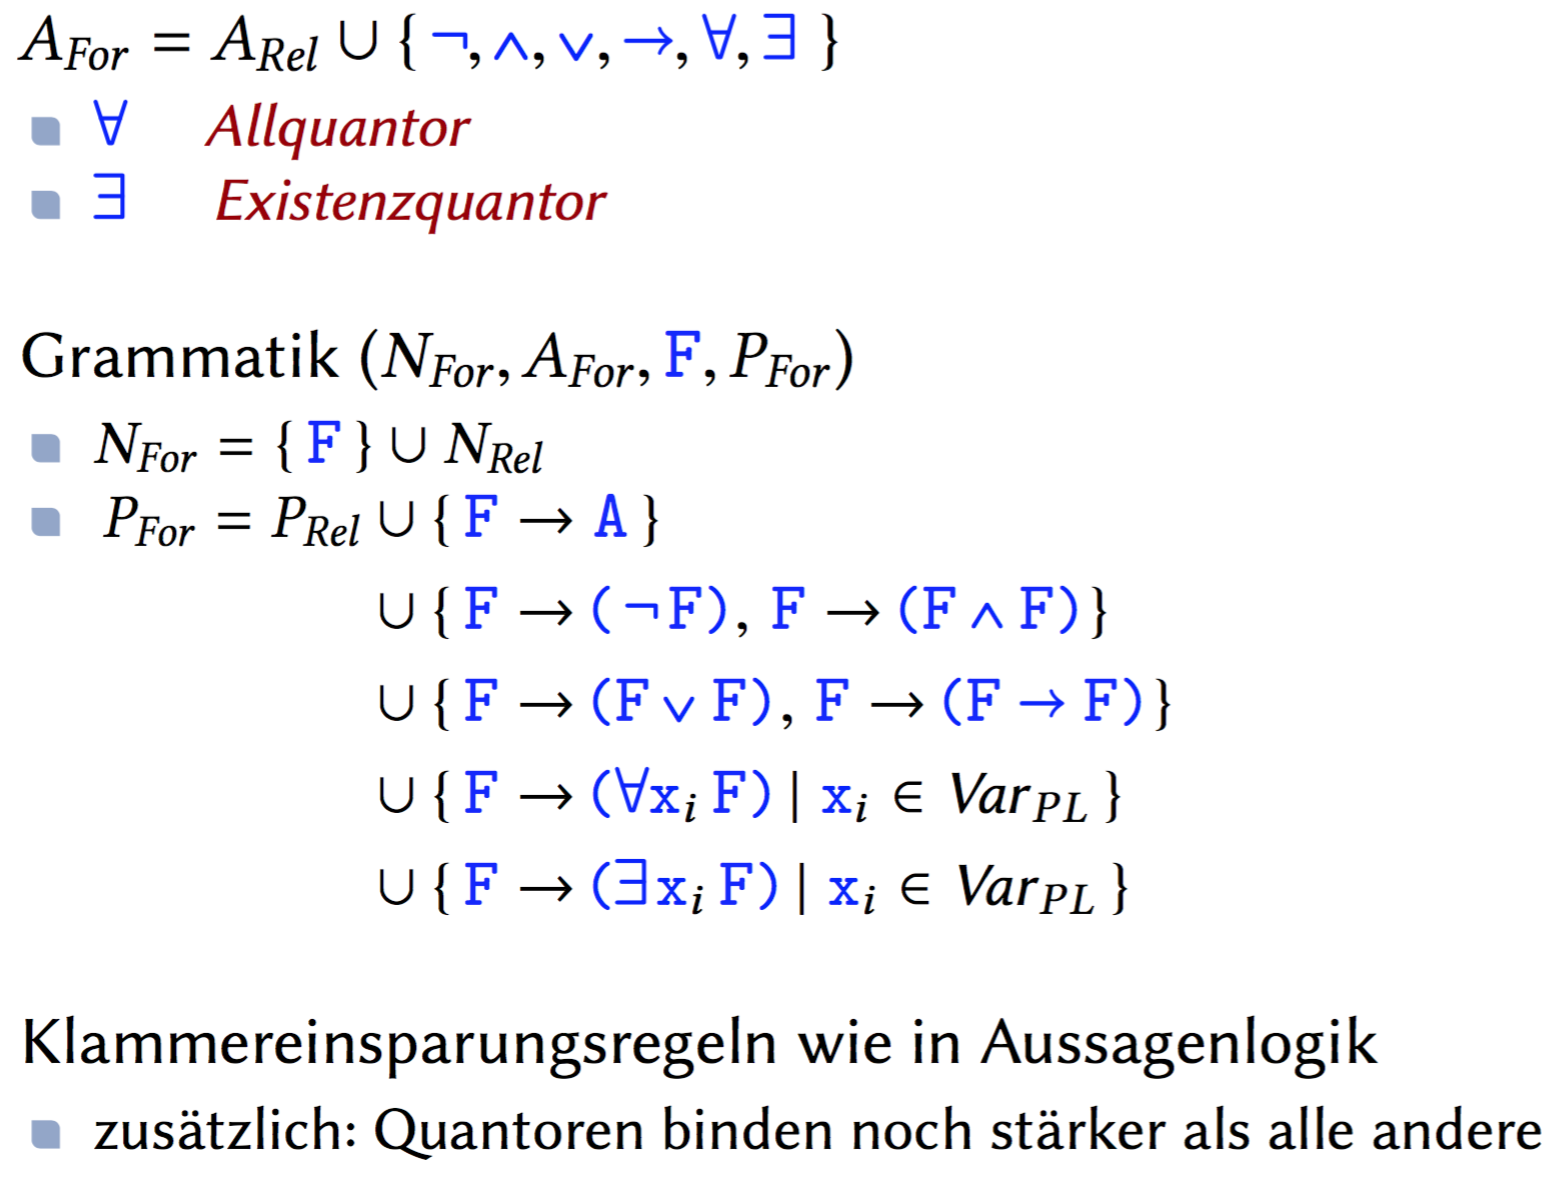
\includegraphics[scale=0.2]{pl/PFormeln.png} \hspace{2em} 
	\end{figure} 
	\end{frame}
}

\begin{frame}{Quiz}
\begin{figure}[h!]
	\centering
	\only<1|handout:1>{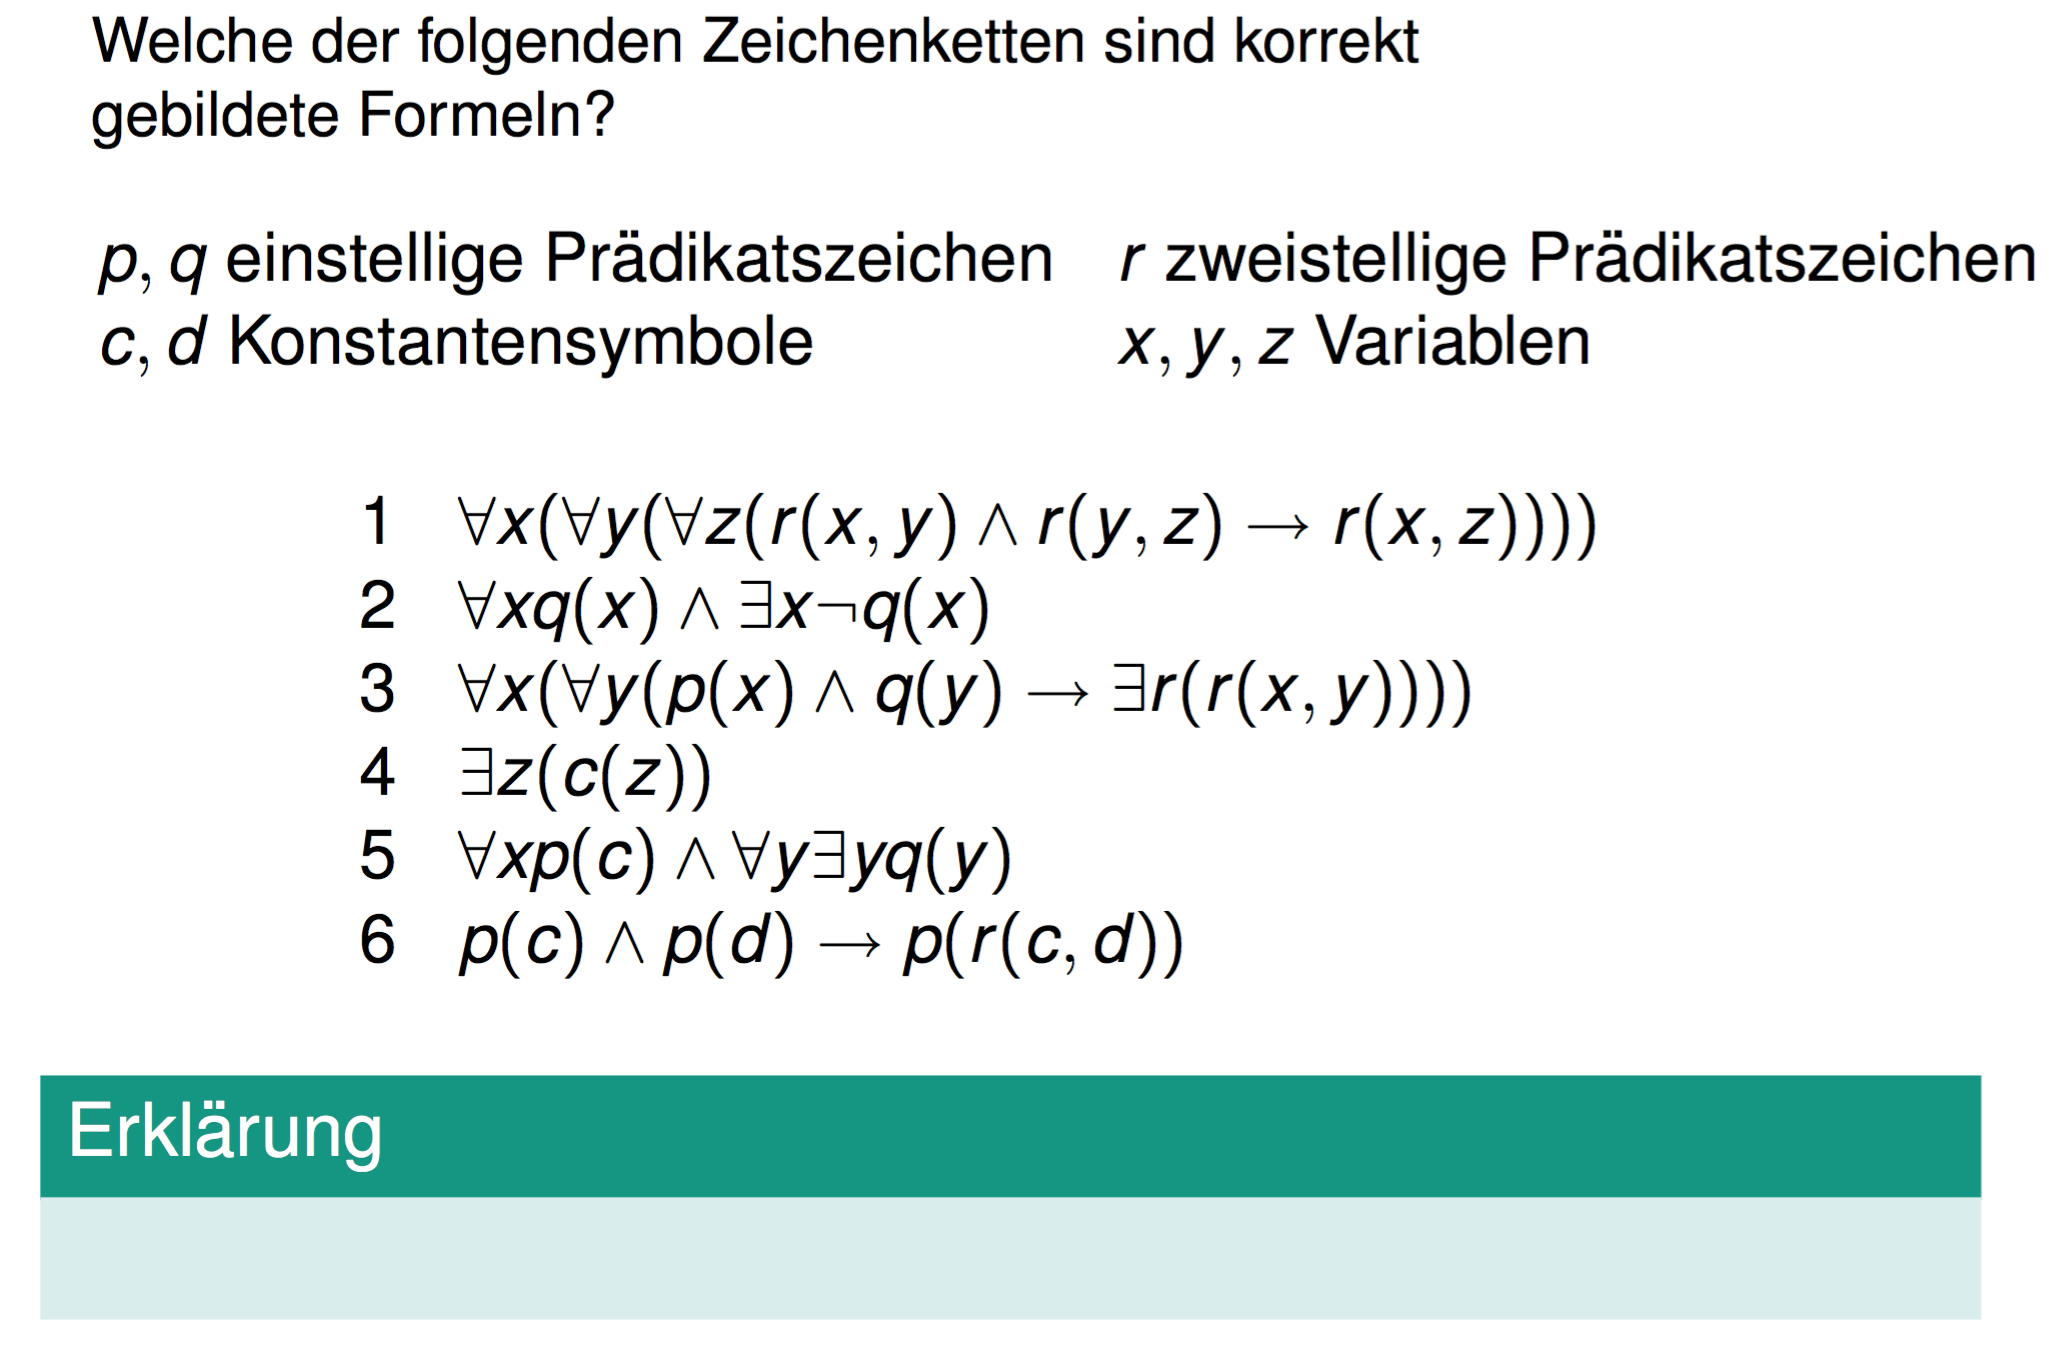
\includegraphics[scale=0.2]{pl/q1.png}}
	\only<2|handout:2>{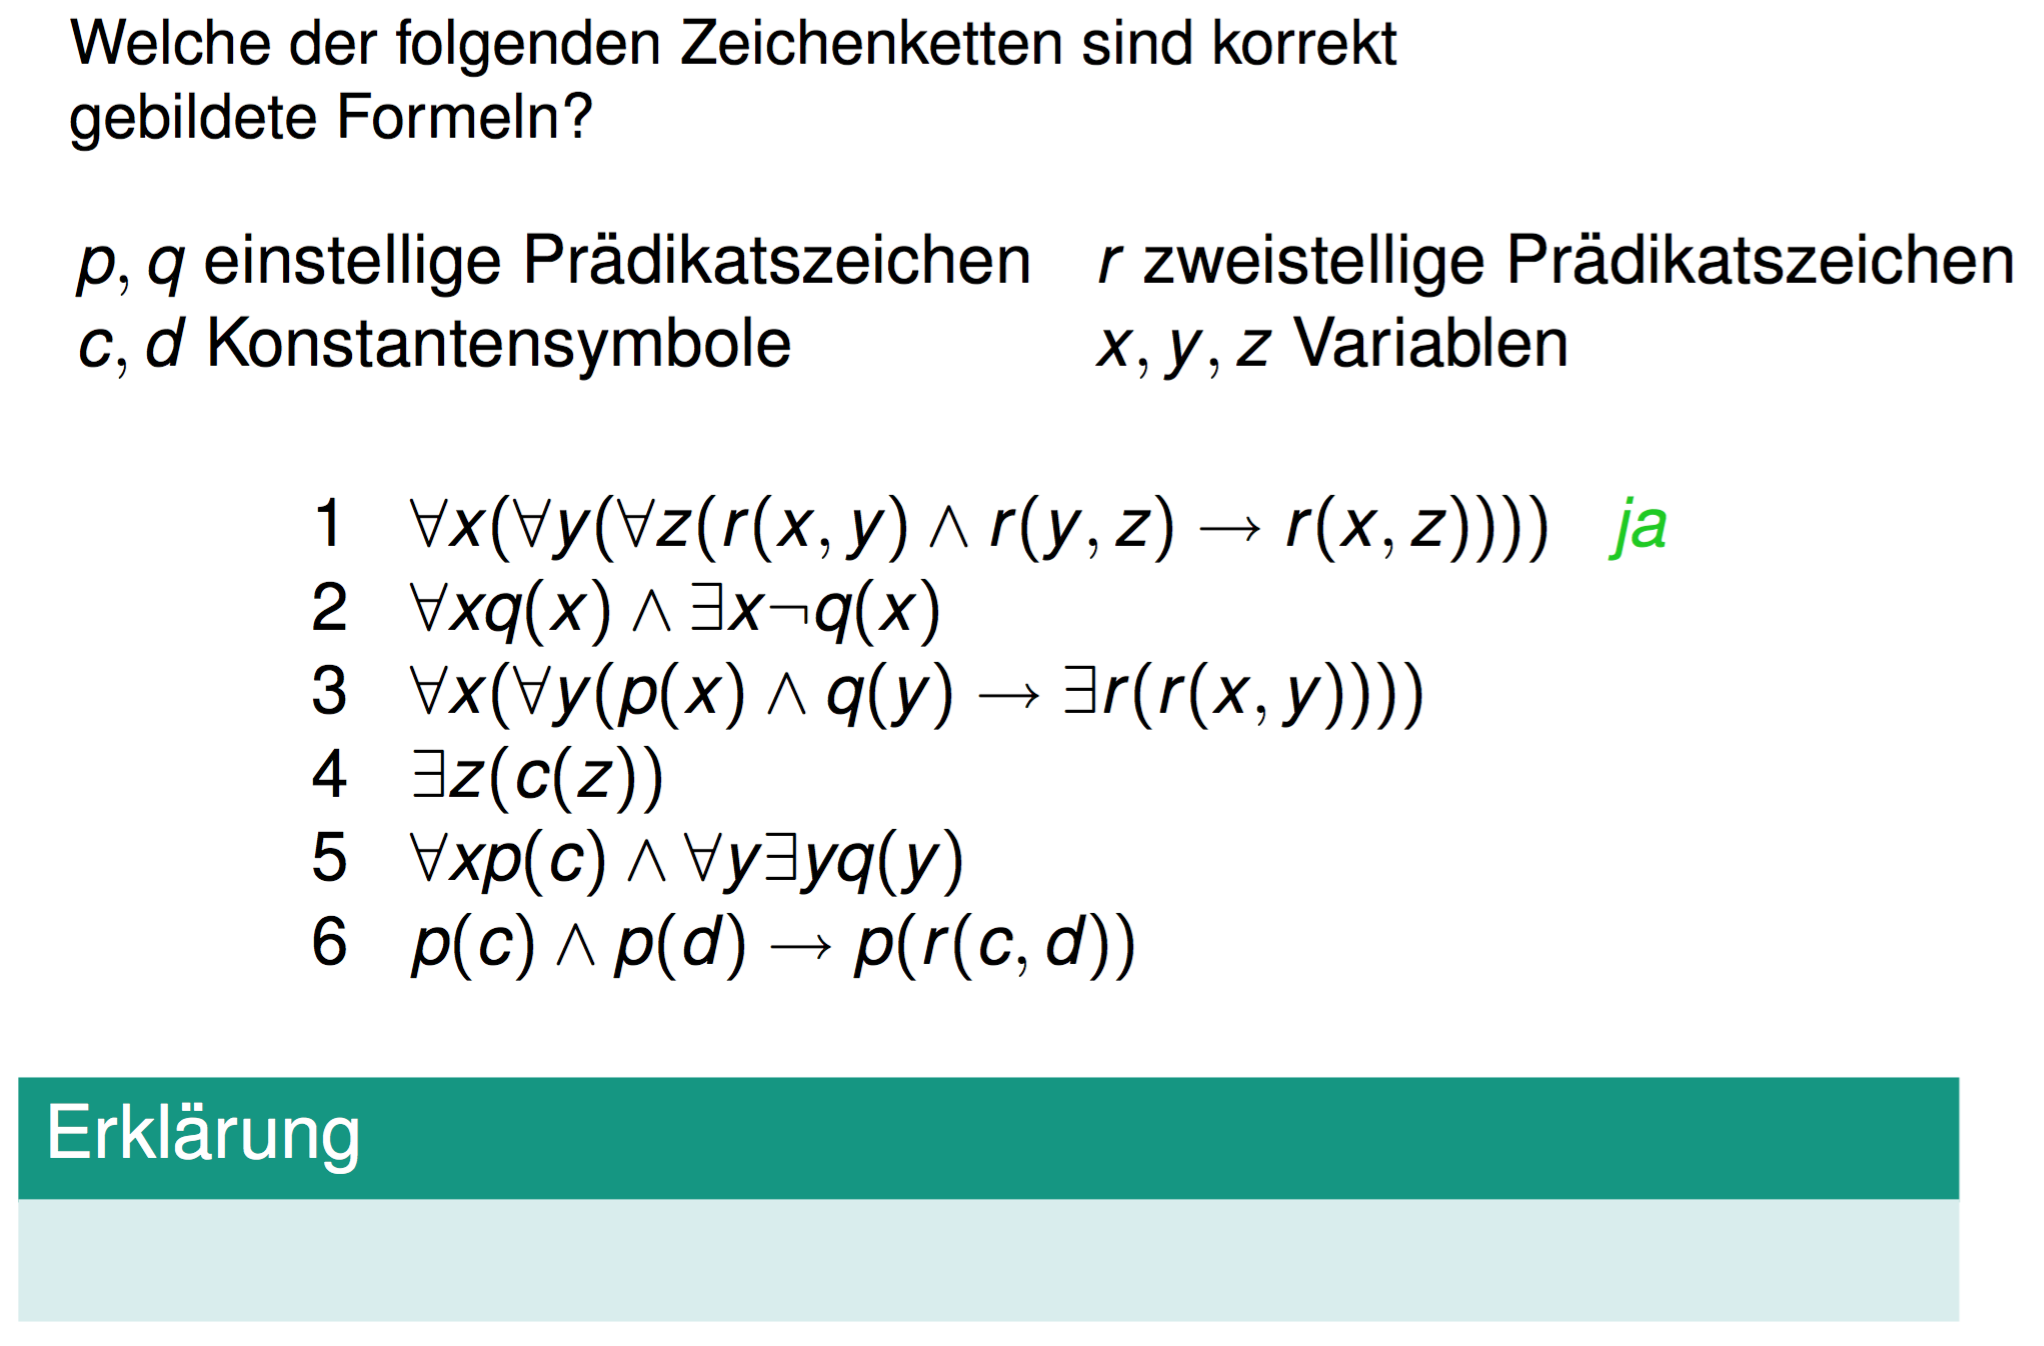
\includegraphics[scale=0.2]{pl/q2.png}} 
	\only<3|handout:3>{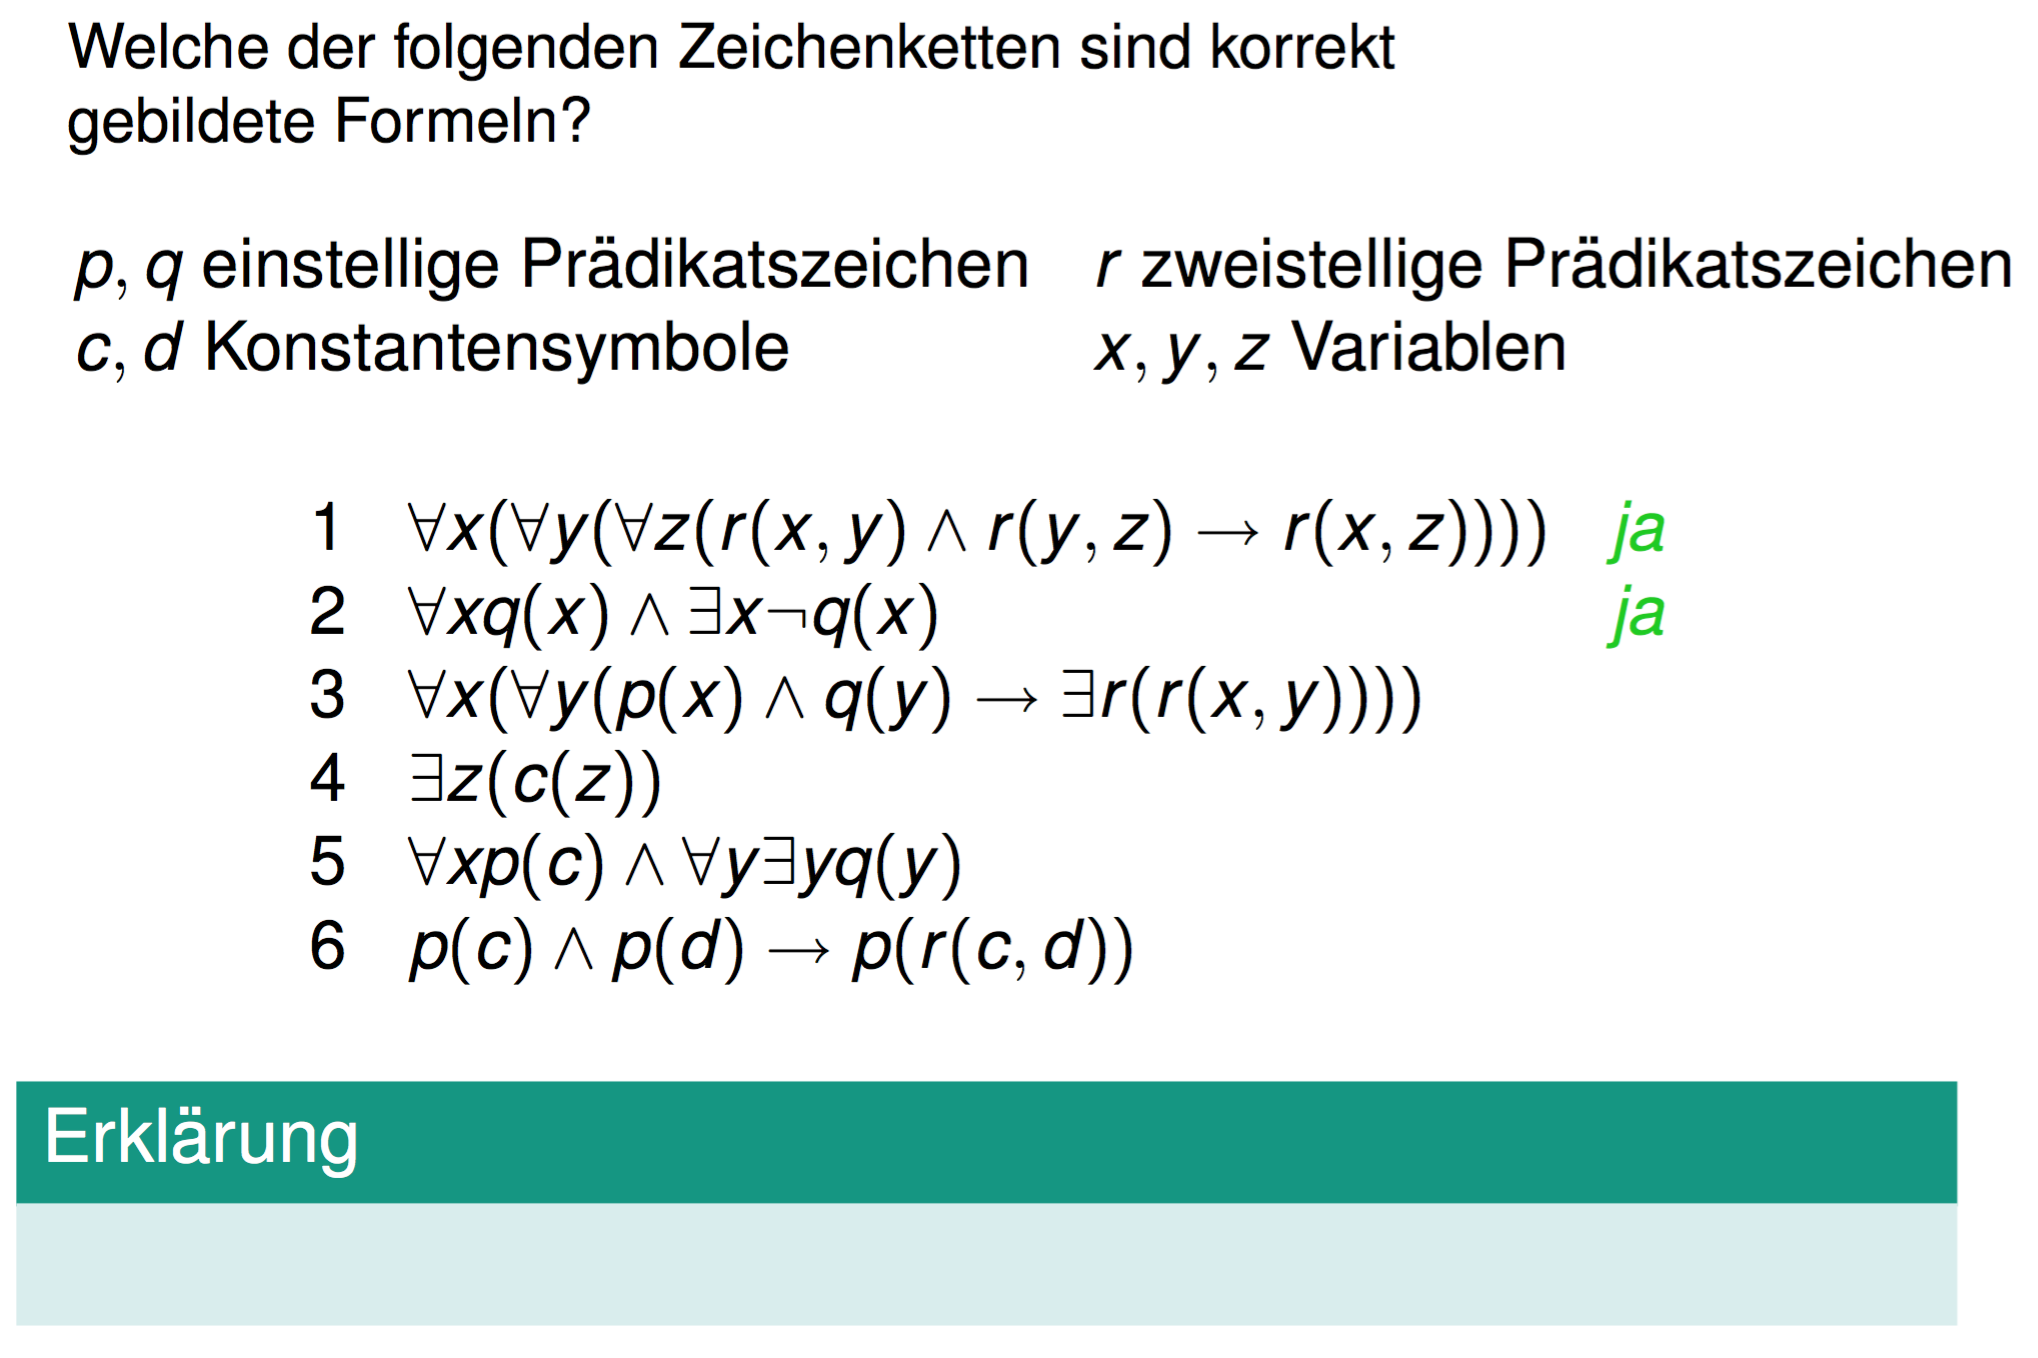
\includegraphics[scale=0.2]{pl/q3.png}}
	\only<4|handout:4>{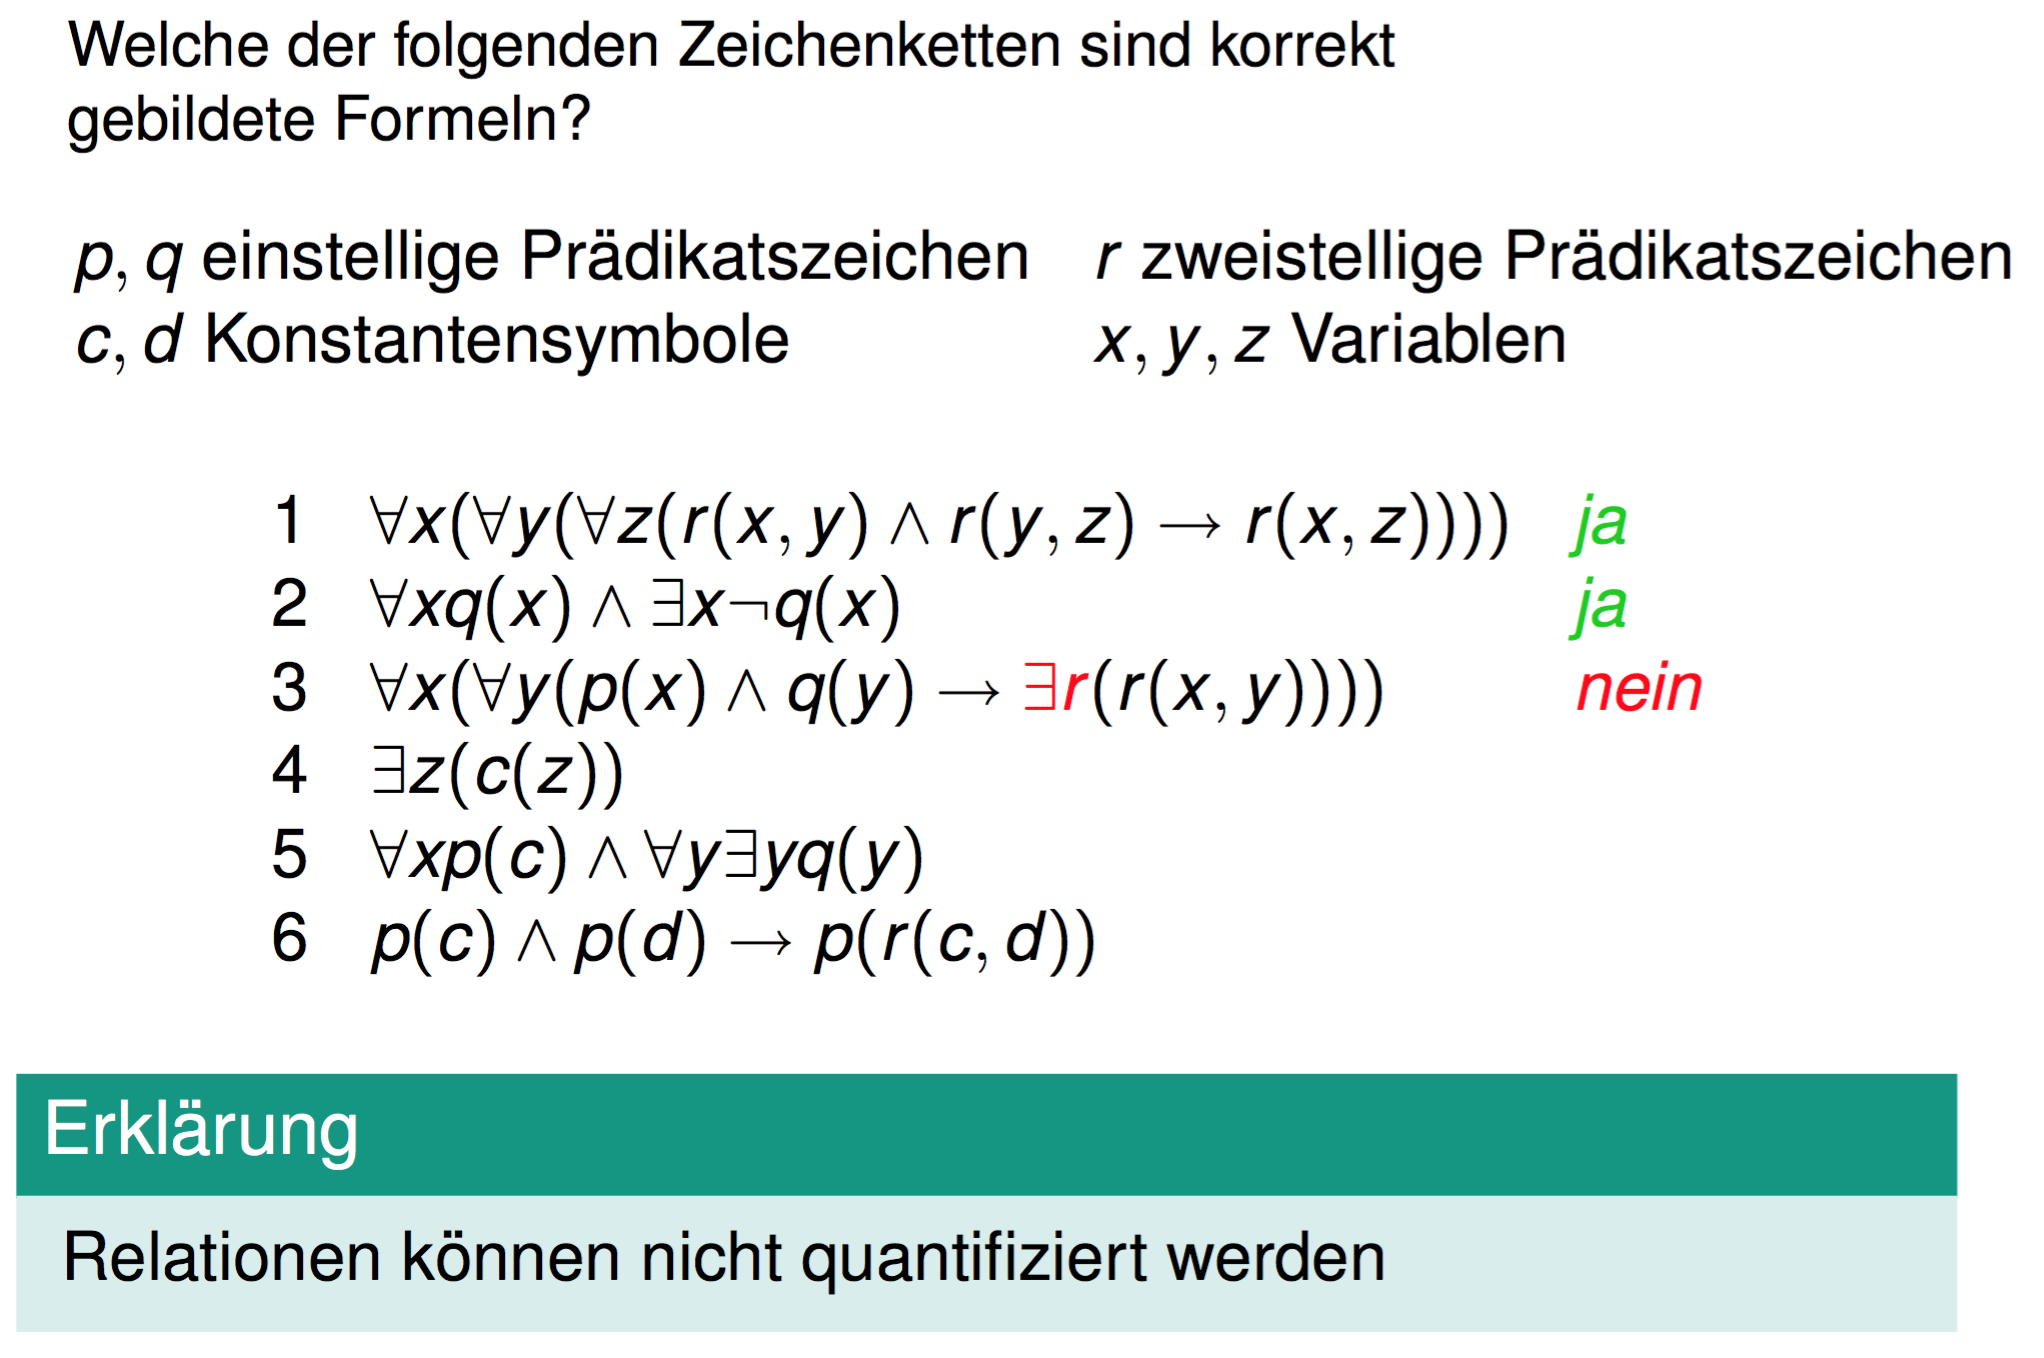
\includegraphics[scale=0.2]{pl/q4.png}}
	\only<5|handout:5>{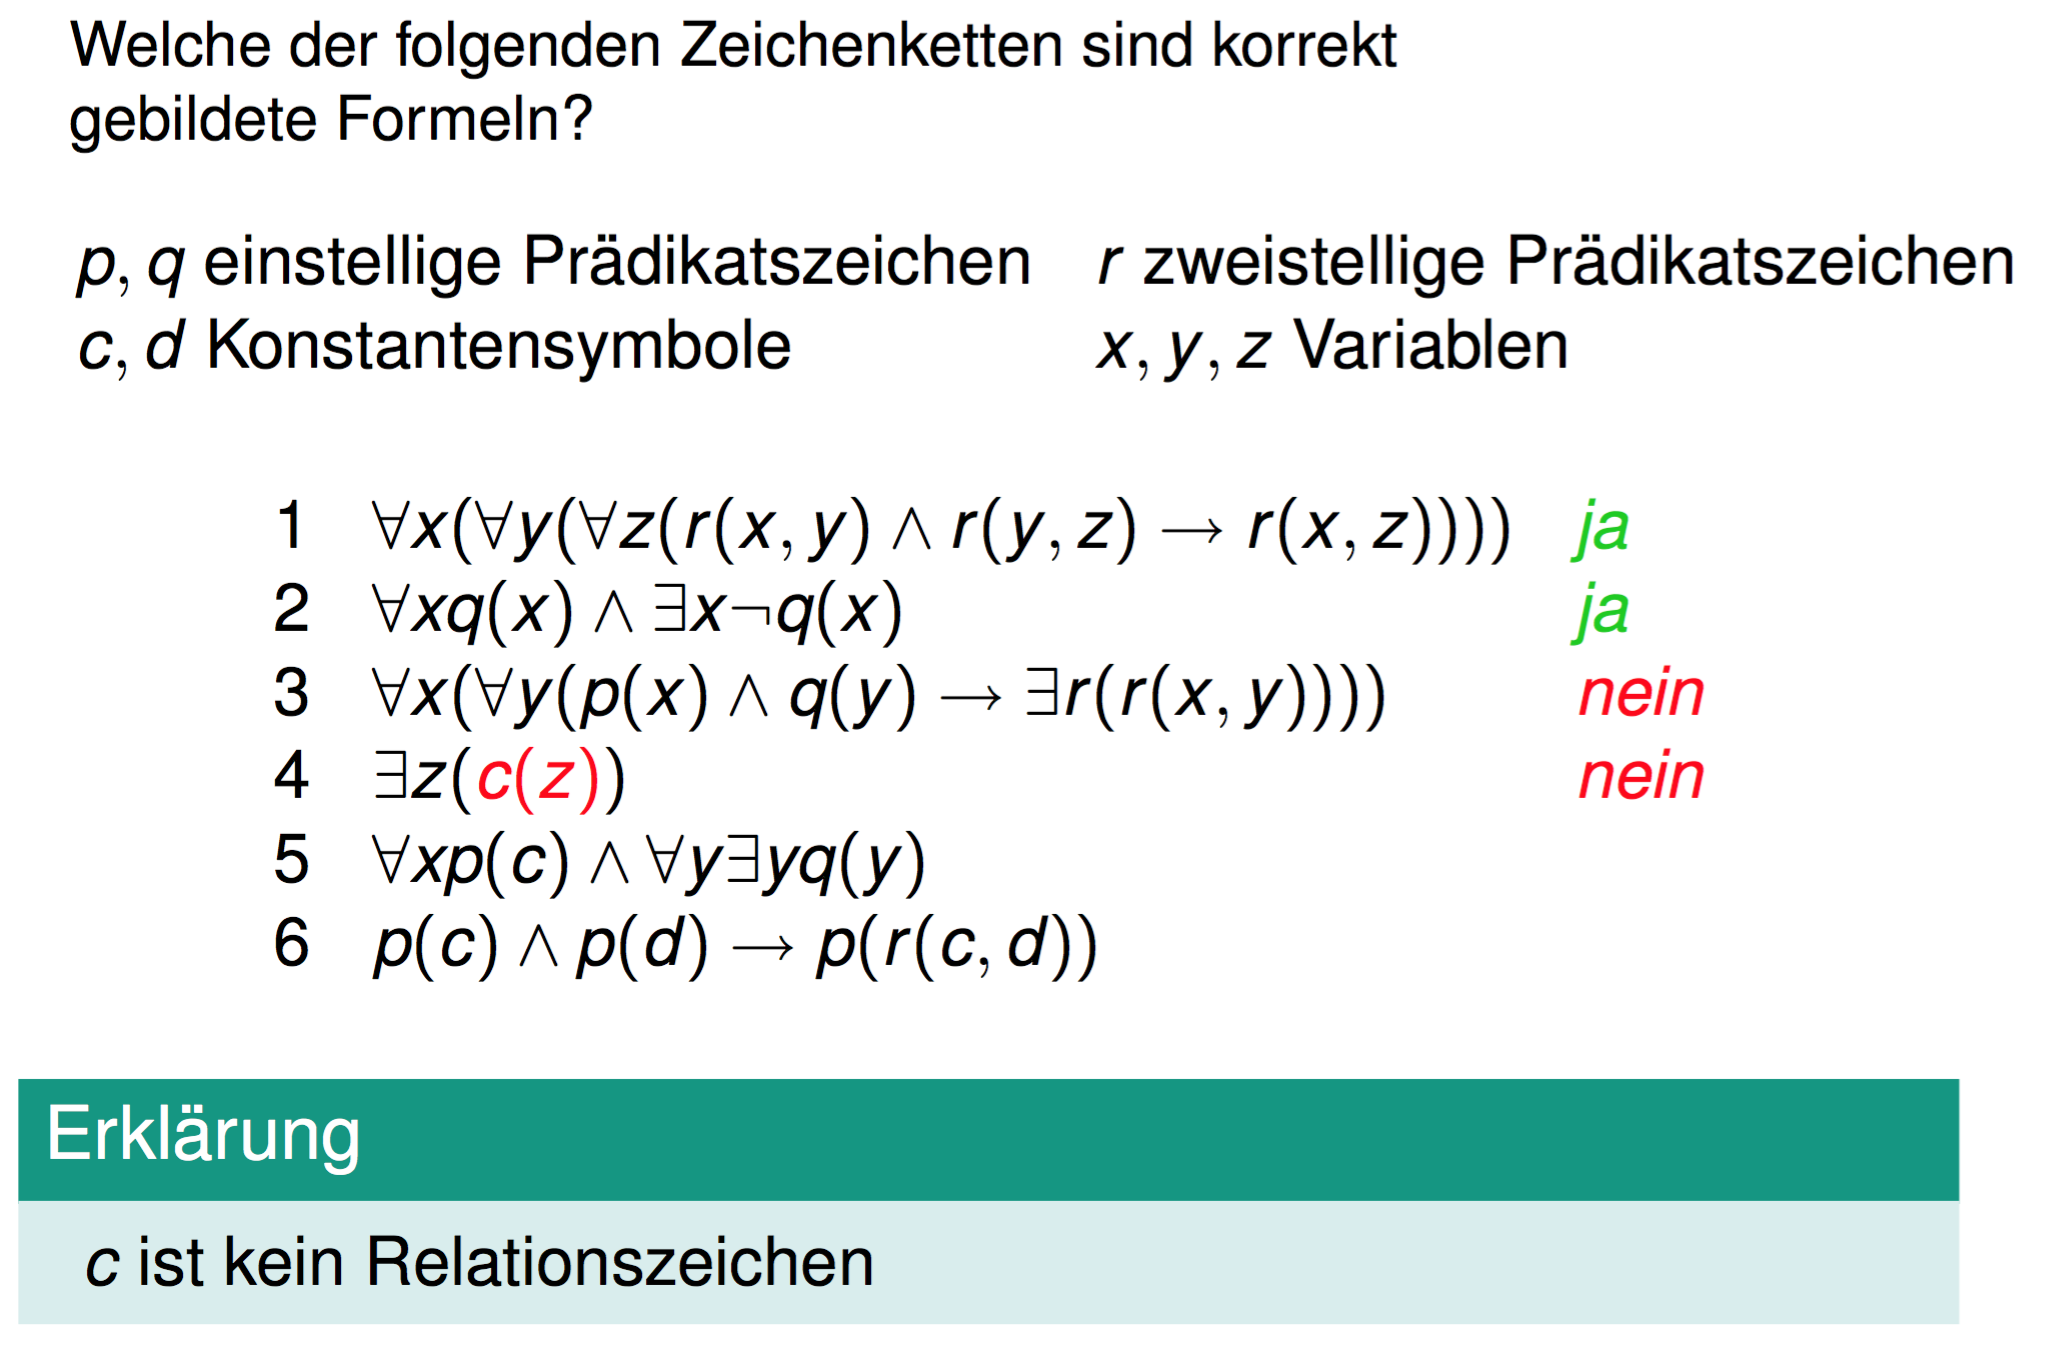
\includegraphics[scale=0.2]{pl/q5.png}}
	\only<6|handout:6>{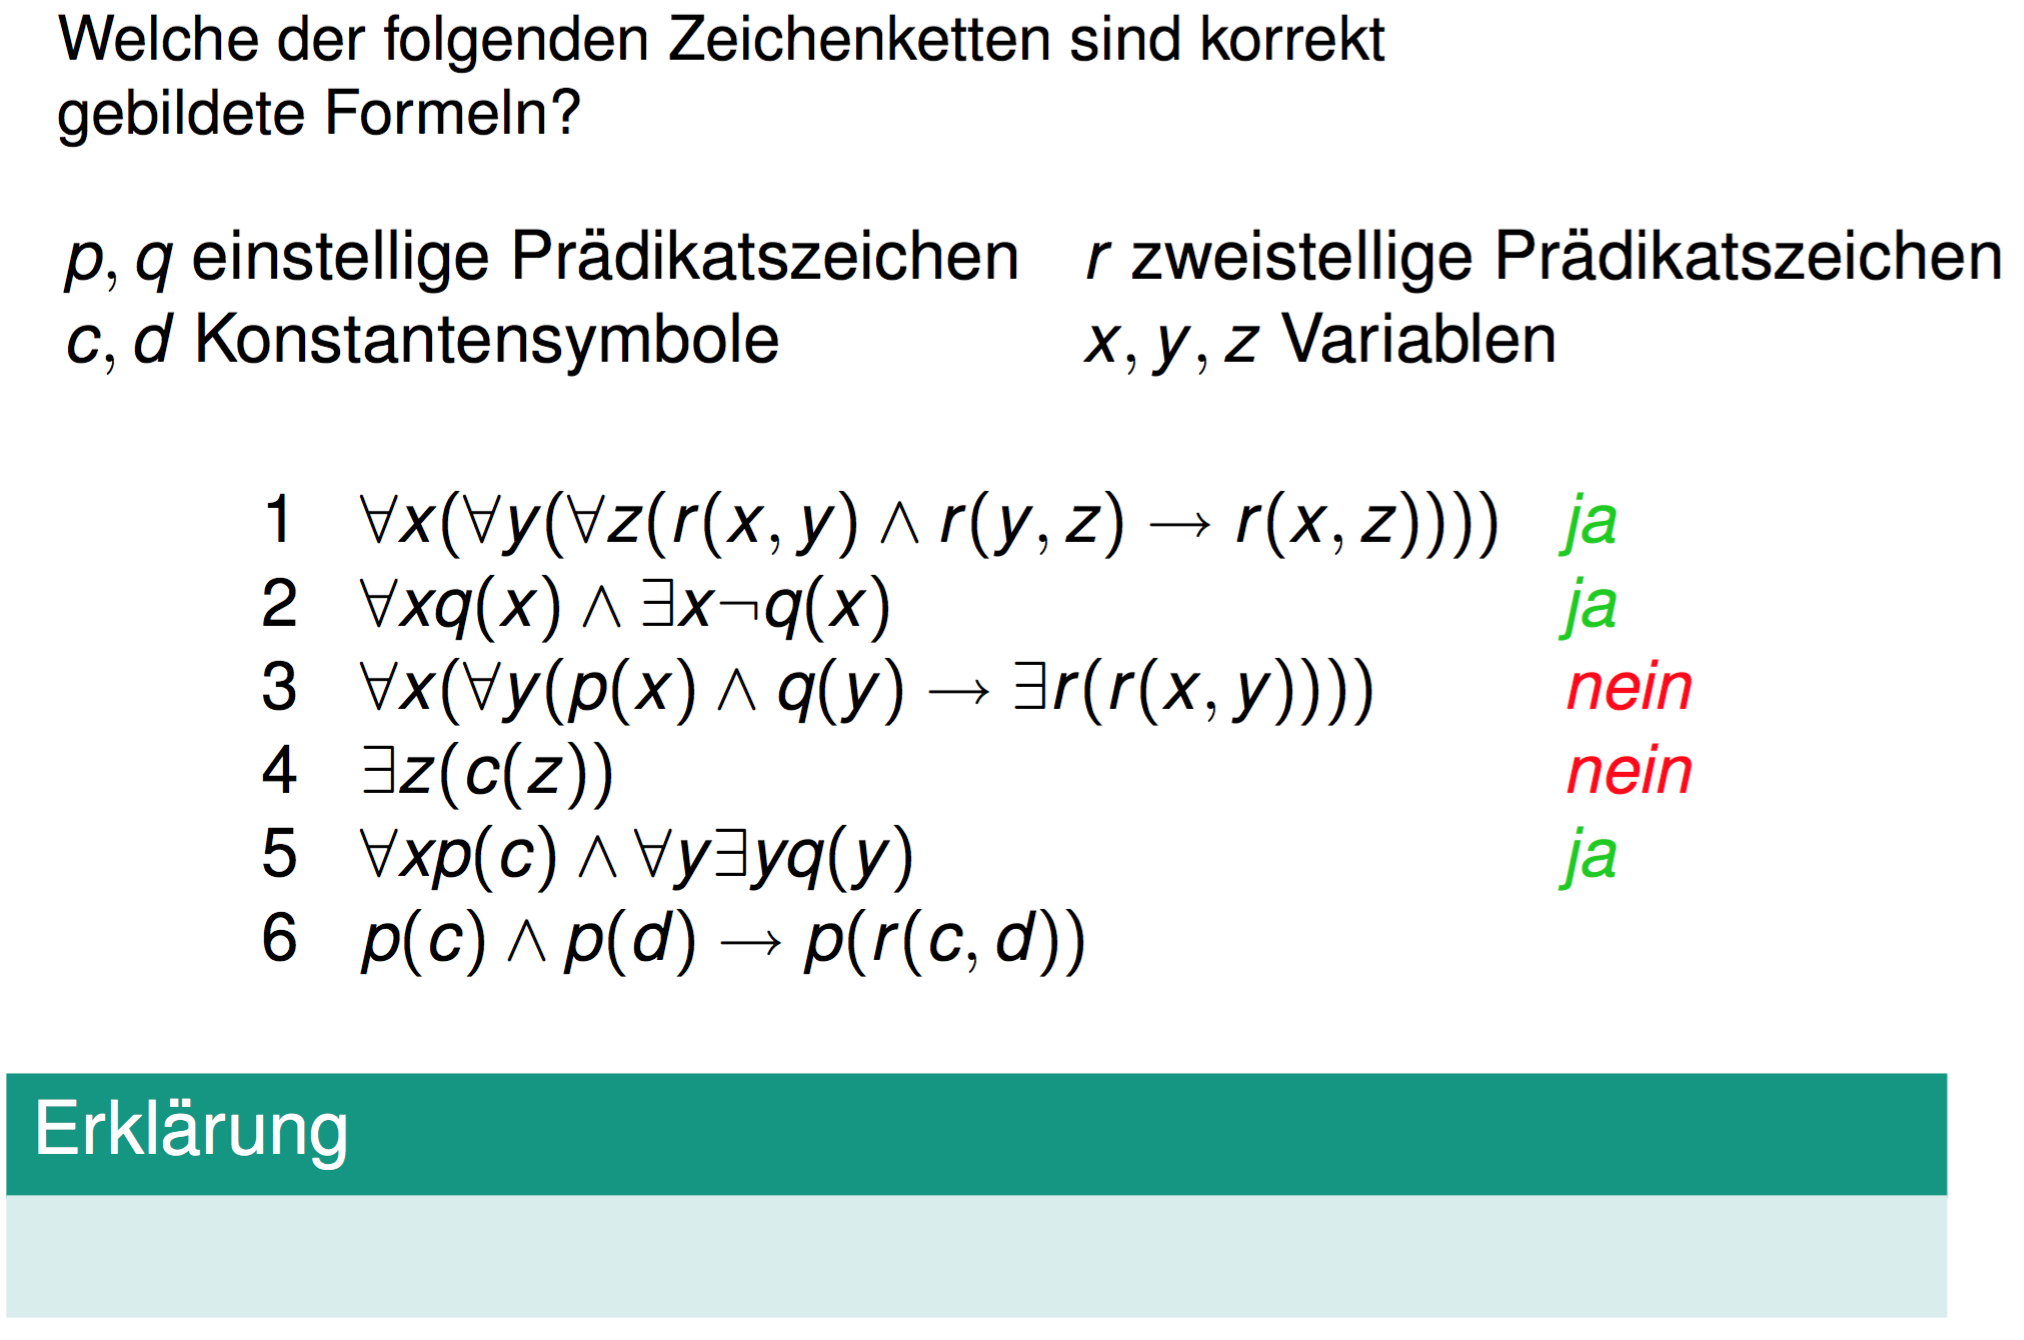
\includegraphics[scale=0.2]{pl/q6.png}}
	\only<7|handout:7>{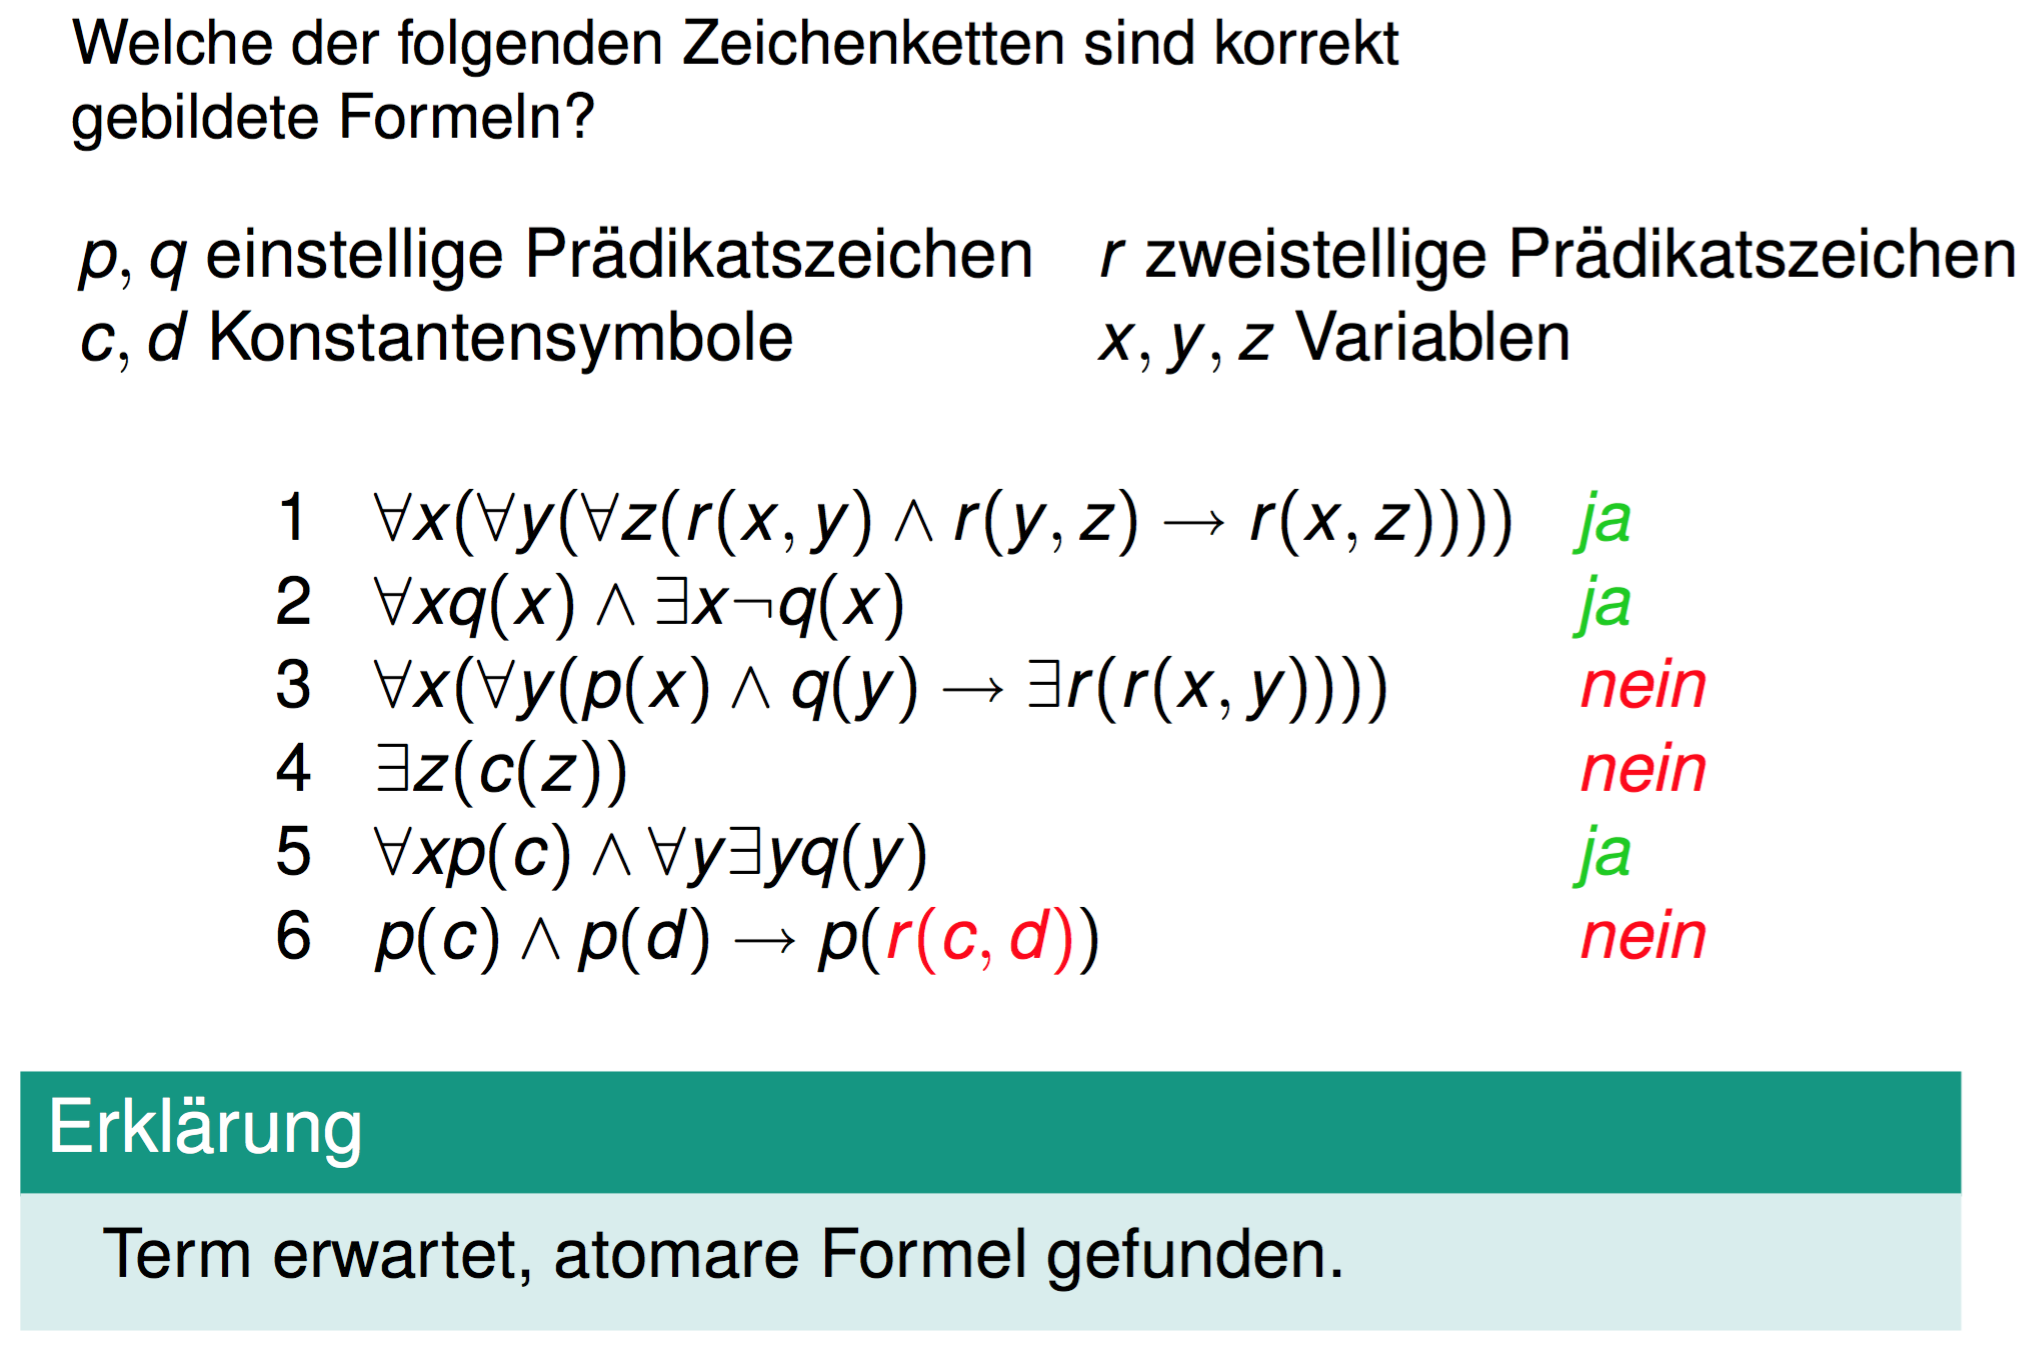
\includegraphics[scale=0.2]{pl/q7.png}}
	\hspace{2em}
\end{figure} 
\end{frame}

\begin{frame}{Aufgabe 2 (WS 15/16, Blatt 7)}
	\begin{block}{Aufgabe}
		Formuliert die folgenden Aussagen als Formeln in Prädikatenlogik:
		\begin{enumerate}
			\item Nicht alle Vögel können fliegen.
			\item Wenn es irgendjemand kann, dann kann es Donald Ervin Knuth.
			\item John liebt jeden, der sich nicht selbst liebt.
		\end{enumerate}
	\end{block}
	
	\visible<2-|handout:2>{
		\begin{block}{Lösung}
			\begin{enumerate}
				\item \qqquad $\plexist \plx {\plka \plfoo{Vogel}{\plka \plx \plkz} \aland \alnot \plfoo{flugfähig}{\plka \plx \plkz} \plkz}$
				\visible<3-|handout:2>{
					\item \qqquad $
					\plexist \plx {\plka \plfoo{kann\_es}{\plka \plx \plkz} \plkz}
					\alimpl
					\plfoo{kann\_es}{\plka \plfoo{knuth} \plkz}
					$
				}
				\visible<4-|handout:2>{
					\item \qqquad $
					\plall \plx {\plka \alnot \plfoo{liebt}{\plka \plx \plcomma \plx \plkz} \alimpl \plfoo{liebt}{\plka \plfoo{John} \plcomma \plx \plkz} \plkz}
					$
				}
			\end{enumerate}
		\end{block}
	}
\end{frame}

\begin{frame}{Freie und gebundene Variablenvorkommen}
	\textbf{Vorkommen} einer Variable in einer PL-Formel: \\
	$G = \plall \word{x\,R(\underline{x})}$ \Impl \word x kommt in $G$ vor. \\
	„Direkt hinter Quantoren“ zählt nicht! \\
	Bsp.: $F = \plall \word{x\,R(c)}$ \Impl \word x kommt \textbf{nicht} in $F$ vor! \\
	\medskip \pause
	
	\textbf{Freie Variablenvorkommen} \quad $\fv(F)$ \\
	Alle, die \emph{irgendwo} in $F$ vorkommen, ohne dass sie quantifiziert sind {\small ($=$ ein Quantor sie einführt)}. \\
	\medskip \pause
	
	\textbf{Gebundene Variablenvorkommen} \quad $\bv(F)$ \\
	Alle, die \emph{irgendwo} in $F$ vorkommen und dabei quantifziert sind. \\
	\medskip \pause
	
	Formel $F$ heißt \textbf{geschlossen} $:\!\!\Gdw \fv(F) = \emptyset$\\
	\medskip \pause
	 
	Beispiel: \\
	$\fv\left(\word{R(\underline{x},\underline{y},c)} \aland \plexist \word x\, \word x \pleq \underline{\word y}  \right) = \set{\word x, \word y}$ \\ 
	\pause
	$\bv\left(\word{R(x,y,c)} \aland \plexist \word x\, \underline{\word x} \pleq \word y \right) = \set{\word x}$
\end{frame}

\begin{frame}{Freie und gebundene Variablenvorkommen}
	\begin{equation*}
	F = \alnot \plexist \plx
	{\plka
		\plE{\plka \plx \plcomma \ply \plkz}
		\alor
		\alnot \plall \plz \plall \plx \plall \ply
		{\plka
			\plE{\plka \plx \plcomma \plz \plkz} \aland \plE{\plka \ply \plcomma \plz \plkz} \alimpl \plx \pleq \ply
			\plkz}
		\plkz}
	\end{equation*}
	
	\begin{block}{Aufgabe 1.1}
		Welche Variablenvorkommen sind frei ($\fv$) und welche gebunden ($\bv$)?\\
		Ist die Formel geschlossen?
	\end{block}

	\pause
	\begin{block}{Lösung}
		Nur die Variable $\fv(F) = \{\ply\}$ kommt frei in $F$ vor.\\
		Genau die Variablen $\bv(F) = \{\plx, \ply, \plz\}$ kommen gebunden in $F$ vor.\\
		Da $\fv(F) \neq \emptyset$, ist $F$ nicht geschlossen.
	\end{block}
	
\end{frame}

\mycomment{
	\begin{frame}{Substitutionen}
		\begin{figure}[h!]
			\centering
			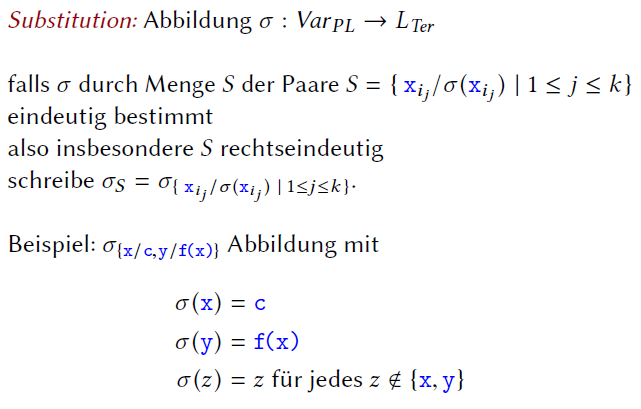
\includegraphics[scale=0.6]{pl/subs.png} \hspace{2em} 
		\end{figure} 
	\end{frame}
}

\begin{frame}{Substitutionen}
	Wollen \textbf{Variablen} (!) durch andere Terme ersetzen. \\
	\impl Eine Substitutionsabbildung $$\sigma_S \from \LFor \functionto \LFor, \, \text{längliche Definition s. VL}$$ wendet Ersetzungen aus $S$ auf einen Term an. \\
	\medskip \pause
	
	Beispiel: \\
	$\sigma_{\set{\word x/\word y}}\left(\word x \pleq \word c\right) = \word y \pleq \word c$. \\
	$\sigma_{\set{\word x/\word{f(c)}}}\left(\word{R(x,y)} \aland \plexists \word y\,\word y \pleq \word x\right) = \word{R(\word{f(c)},y)} \aland \plexists \word y\,\word y \pleq \word{f(c)}$. \\
	\medskip \pause
	
	Mehrere auf einmal: \\
	$\sigma_{\set{\word x/\word y, \, \word y/\word x}}\left(\word x \pleq \word y\right) = \word y \pleq \word x$.
\end{frame}

\begin{frame}{Substitutionen}
	Ersetzt werden nur \textbf{freie Variablenvorkommen}!\\
	Gebundene Vorkommen, also Variablen im Wirkungsbereich eines Quantors, werden \textbf{nicht} ersetzt. \\
	\medskip \pause
	
	Beispiel: \\
	$\sigma_{\set{\word y/\word{f(c)}}}\left(\word{R(x,y)} \aland \plexists \word y\,\word y \pleq \word x\right) = \word{R(x,\word{f(c)})} \aland \plexists \word y\,\word y \pleq \word x$
	
	
	\mycomment{
		\begin{figure}[h!]
			\centering
			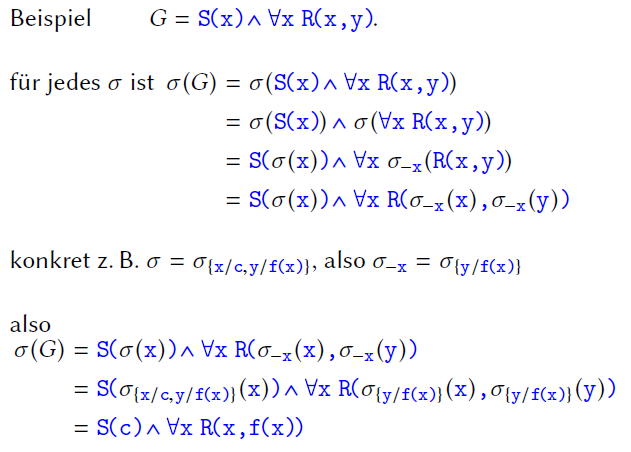
\includegraphics[scale=0.5]{pl/subs_bsp.png} \hspace{2em} 
		\end{figure} 
	}
\end{frame}

\begin{frame}{Substitutionen: Kollisionsfreiheit}
	Bei einer \textbf{kollisionsfreien} Substitution werden keine Variablen \enquote{aus Versehen} gebunden.\\[1em]
	Ersetzen wir eine freie Variable $\word x$ durch einen Term, in dem die Variable $\word y$ frei vorkommt, so darf sich $\word x$ nicht im Wirkungsbereich eines Quantors über $\word y$ befinden.
	
	\pause
	\begin{Beispiel}
		$F = \plall \plx \plka\plx \aland \ply\plkz$\\
		Kollisionsfrei: $\sigma_{\{\ply/\plz\}}$\\
		Nicht kollisionsfrei: $\sigma_{\{\ply/\plx\}}$
	\end{Beispiel}
\end{frame}

\begin{frame}{Substitutionen}
	\begin{equation*}
	F = \alnot \plexist \plx
	{\plka
		\plE{\plka \plx \plcomma \ply \plkz}
		\alor
		\alnot \plall \plz \plall \plx \plall \ply
		{\plka
			\plE{\plka \plx \plcomma \plz \plkz} \aland \plE{\plka \ply \plcomma \plz \plkz} \alimpl \plx \pleq \ply
			\plkz}
		\plkz}
	\end{equation*}
	
	\begin{block}{Aufgabe 1.2}
		Gebt eine Substitution $\sigma$ an, die \emph{nicht} kollisionsfrei für $F$ ist.\\[1em] \pause
		
		Die Substitution $\sigma_{\{\ply/\plx\}}$ leistet das Gewünschte.
	\end{block}
	
\end{frame}


\section{Prädikatenlogik: Semantik}

\begin{frame}{Interpretation}
	\begin{figure}[h!]
		\centering
		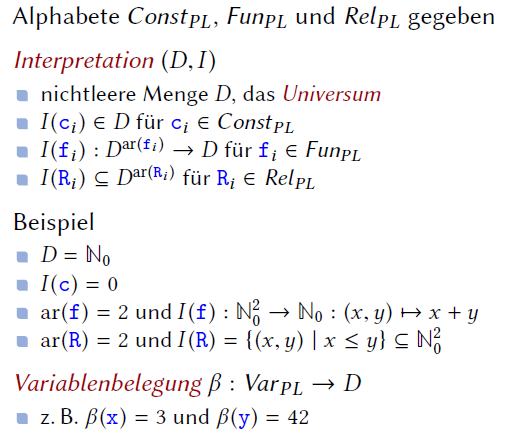
\includegraphics[scale=0.6]{pl/int.png} \hspace{2em} 
	\end{figure} 
\end{frame}

\begin{frame}{Aufgabe 1 (WS 15/16, Blatt 7)}
	  \begin{equation*}
	\alnot \plexist \plx
	{\plka
		\plE{\plka \plx \plcomma \ply \plkz}
		\alor
		\alnot \plall \plz \plall \plx \plall \ply
		{\plka
			\plE{\plka \plx \plcomma \plz \plkz} \aland \plE{\plka \ply \plcomma \plz \plkz} \alimpl \plx \pleq \ply
			\plkz}
		\plkz}
	\end{equation*}\\[1em]
	
	\begin{block}{Aufgabe 1.3}
		Gebt eine Interpretation $(D_1, I_1)$ und eine Variablenbelegung $\beta_1$ so an, dass $val_{D_1, I_1, \beta_1}(F) = \W$ gilt.\\[0.5em]
		
		\visible<2-|handout:2>{Die Interpretation $(D_1, I_1) = (\{ 0, 1 \}, {<})$ und die Variablenbelegung $\beta_1 \colon \VPL \functionto D$, $v \mapsto 0$, leisten das Gewünschte.}
	\end{block}

	\begin{block}{Aufgabe 1.4}
		Gebt eine Interpretation $(D_2, I_2)$ und eine Variablenbelegung $\beta_2$ so an, dass $val_{D_2, I_2, \beta_2}(F) = \F$ gilt.\\[0.5em]
		
		\visible<3-|handout:2>{Die Interpretation $(D_2, I_2) = (\{ 0, 1 \}, {<})$ und die Variablenbelegung $\beta_2 \colon \VPL \functionto D$, $v \mapsto 1$, leisten das Gewünschte.}
	\end{block}
\end{frame}



\section{Prädikatenlogik: Aufgaben}

\begin{frame}{Prädikatenlogische Formeln aufstellen}
	% TODO Übung einbinden
	Vgl. Übung WS 15/16
\end{frame}



\begin{frame}{Weitere Aufgaben}
	Siehe Übung WS 15/16
\end{frame}